\section{Research Questions}

In this section, I outline the problems that I will research. I've broken my proposed work into two main questions, each of which has a series of subquestions.

\subsection{Research Question 1: Technology}

\textbf{What facilitations support the use of Data Science as an introductory context to provide motivation?}

	Data Science is a non-trivial context for introductory learners, due to the difficulty in finding, preparing, and delivering data to students in a pedagogically suitable form.
    Integrating it into a learning experience has already shown to be a tricky experience.
    In this subsection, I've outlined three research questions that I think are get at the heart of these challenges. To explore how to resolve these questions, I propose to build three new pieces of software:
    \begin{description}
    	\item[CORGIS Architecture] An evolution of the existing RTW architecture that handles new use cases and technical issues.
        \item[CORGIS Gallery] An evolution of the existing RTW gallery that makes it easier for students and instructors to find relevant datasets.
        \item[CORGIS Builder] An evolution of the existing RTW builder that makes it easier for developers to prepare data sources.
    \end{description}
    
    The remainder of this subsection motivates the research questions and explains how the proposed technology will help solve them.
    
\subsubsection{RQ 1.1: CORGIS Library Architecture}

\textbf{How can we build and maintain a plethora of divergent datasets, that still ensure students have a uniform experience working with their dataset even in the presence of divergent hardware and datasets?}

	The primary value of the CORGIS project lies in the diversity of its datasets, giving students an empowered opportunity to find a dataset that appeals to their interests and long-term goals.
        The CORGIS library currently has over 35 different datasets, including animal feed data, weather reports, historical disease tracking, and much more.
    However, there is a large burden on the developer to create these datasets, requiring technical, pedagogical, and domain proficiency.
	And once these libraries are developed, they must be maintained: web-based libraries need to stay current with their API, and local libraries need to stay compliant with new hardware.
    Finally, these libraries have to be usable by students no matter what kind of hardware they have and whatever permissions they have on the machine.
    
    Although the RealTimeWeb project greatly simplified the process of creating web-based libraries by using configuration files to generate libraries, this approach has failed to scale.
    Once a library has been generated, it becomes an independent code base with its own copy of the structure needed to access its data -- essentially, we are inlining a tremendous amount of code.
    Worse, the novel features of the library become mired in boilerplate and library specializations.
    For example, consider the differences between the Gutenberg Books library and the Weather library, both of which expose a single function that connects to an online data source and returns a data structure mixing lists and maps: these two libraries are significantly similar except for their initial method to submit the web request and their final method that processes the retrieved data into the proper form.
    When an update is made to the web API, the developer must hunt down these two functions and make modifications, navigating a mess of boilerplate.
    Even worse is when improvements are needed to the core architecture.
    Despite sharing a common general architecture, each library is an independent code base with minute modifications.
    Therefore, a change to the architecture must be percolated to three dozen other codebases.
    
    A second problem with the current architecture is the disorganization of the documentation and metadata that is associated with each library.
    Getting to know an API is a difficult process akin to learning to a new language.
    Supplementary documentation, including tutorials and API references, are necessary.
    The RealTimeWeb project provided tools for documenting the libraries it generated, but these were limited to creating simple API reference materials that were not adaptable to different levels of learners and did not instruct the learner on its use; creating tutorials to use the libraries was a manual, cumbersome effort that was redundant across similar libraries.
    Further, RealTimeWeb had absolutely no tooling to generating supporting documentation related to metadata for the library -- information such as origin of the data, explanation of terminology used, and terms of its use.
    
 The third major problem is that students using our software can have different computational power: seniors might have a laptop from their freshman year, or run an older version of Mac OS.
	Ideally, the students should always be able to run their code quickly and efficiently while developing, without noticeable lag from their programs.
    However, several existing CORGIS libraries suffer greatly from bad caching strategies and poorly sized datasets, resulting in lousy performance that can frustrate beginners.
    A 100 MB library that runs fine on a developers new machine can be treacherously slow on a students' ancient laptop.
    
    \textbf{RQ1.1 Solution: Create a new architecture that simplifies the creation of dataset libraries (whether web-based or local), while being highly maintainable to developers and performant for students.}
    
    Figure \ref{fig-corgis-architecture} shows my vision for the new architecture, highlighting the new components.
    In effect, all of the CORGIS libraries will be represented by one code base with ``plug-and-play'' data.
    These pluggable datasets will also incorporate structured rich metadata with an interface specification to indicate how students can access the data.
    Further, the library will be able to analyze the architectural suitability of the host machine and make intelligent decisions to adapt to the hardware. For example, if the software found that the students laptop had little RAM and a poor processor, it might decide to sample down the dataset, or to process more data on disk.
    
    
    Once the solution is implemented, it will be evaluated based on case studies of creating new datasets and analyzing the work required to update existing datasets. 
    The impact on the students' experience will be analyzed through usability studies: students will be interviewed about their experience learning about the metadata and problems that they encountered while getting to know their dataset.
    More information on these usability studies is given in Research Question 2.1.
    
    \subsubsection{RQ 1.2: CORGIS Builder Architecture}
    
    \textbf{How can we lower the barrier for instructors and domain experts to transform a data source into a classroom ready resource?}
    
    There is still too high a barrier for instructors to transform a data source into a classroom ready tool.
    Although our Real-Time Web Tool simplifies the process of connecting to web-based APIs, it has no features for simpler local datasets. 
   Preparing a dataset is an adhoc process of converting between data formats (e.g., JSON, CSV, SQL, etc.) into something manageable, requiring decisions about what fields and instances to keep, how the data should be structured hierarchically, what type fields should be, and how data should be pre-aggregated for students.
   
   A further limitation is that the RTW Builder has no support for the process of building data caches.
   Instead, the instructor has to use the individual library to build up data caches using a poorly documented internal tool.
   This tool works in a cumbersome ``VCR recording''-style, where the user runs the queries they're interested in retaining in real-time. 
   There is no way for the instructor to create artificial data caches matching their use case, without resorting to writing their own completely custom scripts.
    
    Finally, different datasets have wildly varying structure depending on the nature of their data.
    A student working with social media data may find the data to be recursive or tree-structured, as opposed to a student with more tabular data working on sports statistics.
    Although this may be expected and natural, it is not desirable or necessary for students to have wildly divergent experiences with learning the structure of their data. 
    If there is a uniform shape to the data, the instructor can have confidence and knowledge in providing technical and pedagogical support, no matter which student they are helping.
    Inversely, they can give a more uniform lecture that is accurate for all of the students.
    
    \begin{figure}
\begin{center}
\tikzset{
    bnode/.style = {   
        align=center, draw,
        rectangle split, rectangle split horizontal,
				rectangle split draw splits=false
    }
}
\begin{minipage}{.4\textwidth}
\begin{tikzpicture}
    \node[align=center, draw] (root)
		  {List of}
		;
		\node[bnode, below=of root,rectangle split parts=3]
       (middle)
       {	\nodepart{one}
					Dictionary of:
					\nodepart{two}
          ``city'' ,
					\nodepart{three}
					``temperature''
					};
		
    \draw (root) -- (middle);
    \draw (middle.two south) -- +(0, -1) node[draw, anchor=north](q) {string};
    \draw (middle.three south) -- +(0, -1) node[draw, anchor=north](q) {integer};
		%  +(0,-1) 
\end{tikzpicture}
\begin{center}
\textbf{(A) List of Weathers}
\end{center}
\end{minipage}
\hspace{1cm}
\begin{minipage}{.4\textwidth}
\begin{center}
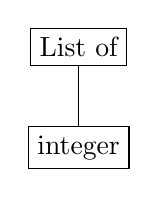
\begin{tikzpicture}
		\node[align=center, draw] (root)
		  {List of}
		;
		
    \draw (root) -- +(0, -1) node[draw, anchor=north](q) {integer};
		%  +(0,-1) 
\end{tikzpicture}
\end{center}
\begin{center}
\textbf{(C) List of Temperatures}
\end{center}
\end{minipage}
\vspace{1cm}
\tikzset{
    bnode/.style = {   
        align=center, draw,
        rectangle split, rectangle split horizontal,
				rectangle split draw splits=false, rectangle split parts=4
    }
}
\begin{tikzpicture}
		\node[bnode]
       (root)
       {	\nodepart{one}
					Dictionary of:
					\nodepart{two}
          ``blacksburg'' ,
					\nodepart{three}
					``newark'',
					\nodepart{four}
					``venice''
					};
		
    \draw (root.two south) -- +(0, -1) node[draw, anchor=north](q) {integer};
    \draw (root.three south) -- +(0, -1) node[draw, anchor=north](q) {integer};
		\draw (root.four south) -- +(0, -1) node[draw, anchor=north](q) {integer};
		%  +(0,-1) 
\end{tikzpicture}

\begin{center}
\textbf{(B) Dictionary of Weathers}
\end{center}

\end{center}
\caption{The same dataset can be structured differently according to the lesson at hand}
\label{data-maps-weather}
\end{figure}
    
    
\begin{figure}
    \begin{center}
    	\includegraphics[width=.5\linewidth]{images/corgisDatasetArchitecture.png}
    \end{center}
    \caption{The proposed CORGIS Dataset Library Structure}
    \label{fig-corgis-architecture}
\end{figure}
    
    \textbf{RQ 1.2 Solution: An evolution of the RTW Online Building tool to make it even easier to prepare a JSON/CSV data source into a library.}
    
    This new version of the Online Building Tool will have features to reshape and organize a dataset, including ways to create data caches and artificial reworkings of the dataset according to instructor-supplied constraints.
    Specifically, the tool will be able to work with several different data formats, including CSV, JSON, SQL, and TXT, and be able to write definitions to connect to online APIs.
    Instructors will be able to write commands and queries to transform the data according to certain common functions or by using a regular query syntax.
    Figure \ref{data-maps-weather} demonstrates how the same dataset can be parred down into different structures.
    Specifically,  the tool will be able to manipulate datasets to have a desired shapes by restructuring the data according to certain common templates and high-level instructions given by the instructor.
    For example, consider a dataset of car makes and models over years with the columns ("year", "make", "model", "company"); this dataset could be grouped by year in order to make it easier for students to create bar charts in matplotlib (which would otherwise require the student to write grouping code).
    The other crucial new feature of the builder will be the ability to specify constraints and rules to generate artificial data for testing or to expand a data source, such as fake weather reports for the weather library.
    This use of mocking is a powerful way to provide more controlled learning experiences for learners.
    The output of the tool will be pluggable datasets suitable for the CORGIS architecture, rather than specific language bindings.
    
    \subsubsection{RQ 1.3: CORGIS Gallery}
    
    \textbf{How can we support students' and instructors discovery of their data source?}
    
	Instructors have a choice to assign students a specific library, a choice of libraries, or to give students freedom to choose their own library.
    There are motivational and pedagogical trade-offs to consider, but this decision lies with the instructor.
    The goal of the CORGIS library is to allow the instructors to be as flexible as they want in assigning a dataset.
    
    Currently, the list of CORGIS libraries is represented as a flat list of the libraries' names in a wiki structure \footnote{\url{http://think.cs.vt.edu/wiki/index.php/Category:Library}}. Each library has an ad-hoc page of information which may or may not include code examples, library description, and a link to the source code. As the selection grows, this informal representation becomes more and more inadequate for finding a suitable library and learning more about its nature. Originally, the gallery was a dynamically generated page based on a separate specification of the libraries (separate from the libraries themselves) -- this was too difficult to keep in sync with the libraries as they changed. The Wiki technology was adopted to make it simpler to make quick updates, but that just exacerbated the problem of keeping the library documentation up-to-date.
    
    \textbf{RQ 1.3 Solution: An enhancement to the RTW Online Gallery to make it more interactive and guiding for students to discover their datasets}
    
    I propose to make a new version of the RTW Gallery for the CORGIS project with three design goals:
    \begin{enumerate}
    \item Support instructors and students finding a suitable dataset. Provide features for both browsing and searching for libraries, especially for students who might have limited domain knowledge.
    \item Support students looking up information about a library. Provide accessible information about the origin of the data source, the abstractions that it uses, citation data, information about the data's structure and fields, the interface exposed to access the data, any important limitations and features of the dataset, and other metadata relevant to the learner.
    \item Keep the publicly available information of a dataset in sync with the datasets source. In particular, make it easy for developers to update the dataset or the metadata for the dataset, without requiring interaction with the server.
    \end{enumerate}
    
    In the case of the first two design goals, success will be measured qualitatively through the motivation and usability interviews described in section 7.2.
        
\subsection{Research Question 2: Impact}

\textbf{How do the student-driven data context and scaffolds impact students' motivation and engagement?}

	In this proposal, I seek to study how the context and facilitations affect students self-reported motivation and the more quantifiable outcomes of engagement.
    The data to answer these questions will be collected over the course of a semester in an undergraduate Computational Thinking course. Students will be surveyed twice (pre-/post-) and interviewed individually about their experiences. Performance data will be collected in the course.
    
    \subsubsection{RQ 2.1: Motivation}
    
    \textbf{What is the impact on motivation?}
    
    As previously described, the MUSIC Model states that Motivation comes through five different avenues: sense of empowerment (agency), sense of usefulness, sense of success (self-efficacy), interest, and a sense of being cared for.
    I seek to understand how a students' motivation to engage in the course changes over the semester, particularly in relation to the content, context, and scaffolds of the course. 
    
    \textbf{RQ 2.1 Solution: Measured through self-reported quantitative surveys and qualitative interviews}
        
    The MUSIC model has an associated instrument named the Music Model of Academic Motivation Instrument (MMAMI) that can be used to quantitatively measure these attributes, but MMAMI will not be used in this study; the instrument is 26 questions long and is more targeted towards formative, holistic course revision than measuring the motivation attributable to course components.
    For instance, the instrument queries students about ``the coursework'', and making the survey more specific extends the length too far.
    Instead, a custom survey based directly on the MUSIC model will be used to collect quantitative data about the students' motivation.
    This survey is given at the start of the semester (using the future-tense) and the end of the semester (using the past-tense).
    
    The complete text of this survey is included in Appendix A. However, to summarize the survey, there are two main parts.
    The first half is five series of five 7-point likert statements (Strongly Disagree -> Strongly Agree). Each series relates to a different part of the MUSIC model (``I believe it will be interesting to...''), and each likert statement relates to a different part of the course:
    \begin{itemize}
    \item "... learn to write computer programs" - course content related to algorithms.
    \item "... learn to work with abstraction" - course content related to abstraction.
    \item "... learn about the social impacts of computing" - course content related to social ethics.
    \item "... work with real-world data related to my major" - course context related to data science.
    \item "... work with my cohort" - course scaffold related to the collaborative nature of the course.
    \end{itemize}
    
    These five elements were chosen as some of the most clear and important elements of the course that would be visible and understandable to a student at both the beginning and ending of the course.
    Although there are other course elements that would be desirable to gather data on (e.g., the block-based environment), there is a limited number of questions that we can ask students. 
    These questions should be considered formative, as new elements might be added in future semesters.
    For now, these questions get at the three main course content objectives, the course context, and one of the most visible scaffolds available to students.
    
    The second half of the survey instrument has five open-ended qualitative questions relating to the components of the MUSIC model, phrased to ask for particularly extreme examples of motivating and demotivating aspects: for example, the first question is ``So far, what parts of the course seem particularly interesting or boring to you?''. While the first half of the survey will give structured data about the components of the course, this section will give rough data about the ``stand-out'' parts. The data collected will be analyzed using a grounded method to establish recurring themes in the course components -- for instance, a large percentage of students might report that the block-based environment made them feel particularly successful.
    
    The data gathered using this instrument will be used to answer the following specific subquestions:
    
    \begin{enumerate}
    \item What are students initial, self-reported attitudes and expectations entering the course?
    \item How does students' motivation change over the course of the semester?
    \item What course components are particularly effective or not effective at providing motivation?
    \item Do different course components affect different aspects of motivation in different ways (e.g., scaffolds would be expected to affect success, but do they also have an impact on sense of usefulness or interest?)
    \end{enumerate}
    
	In addition to the survey, a sample of students will be interviewed near the end of the semester in order to gather rich qualitative data specifically on the use of the data science context (as opposed to the course components in general).
    I will attempt to select students to gather a representative distribution of the population as a whole, but this will be limited by the volunteer nature of the interviews.
    Questions will be asked relating to the students motivation towards the dataset, but also about the usability of their experience.
    The interview will be conducted over a period of roughly 30-45 minutes and will be audio recorded to make analysis easier.
    
    The complete protocol for the interview is given in Appendix B. The interview will begin an introduction describing the overal goal, and some questions about the current status of the student. Then they will be questioned on their dataset in general and in relation to the five components of the music model (e.g., ``What aspects of your dataset did you have control over?''). Finally, they will be asked an open-ended question about the dataset.
    
    The data collected in the survey will be used to answer the following subquestions:
    
    \begin{itemize}
    \item What aspects of the dataset experience affected the students' motivation?
    \item Do the students understand how to use the dataset?
    \item Do students generally expect the dataset to be authentic and relate to the real-world?
    \item How do students view the data science context in comparison to the rest of the course?
    \end{itemize}
                
    \subsubsection{RQ 2.2: Engagement}
    
    \textbf{What is the impact on engagement?}
    
    Within this proposal, I define engagement as the outcomes of motivation, as opposed to motivation itself which is internal and non-observable.
    There are a wide range of outcomes that can be classified as potential outcomes of engagement. 
    These outcomes represent desirable behavior from students that should be affected by their internal motivation.
    I will analyze students engagement in order to find what can be predicted by their motivation.

    \textbf{RQ 2.1 Solution: Measured through observable outcomes and some self-reported information}
    
    In order to do this analysis, I will collect several different outcomes of their observed behavior.
    The following is a list of the outcomes I will be measuring, and their source:
    
    \begin{description}
    \item[Attendance] Measured as a numeric value indicating how many classes they attended. This is a normal part of the course metrics, since attendance influences a students' grade.
	\item[Procrastination] Measured as a number indicating how many times the student handed in an assignment late.
    \item[Assistant Observations] Measured as two numbers that reflect the students' primary teaching assistant assessment of the students' motivation and ability. This will be collected near the end of the semester.
    \item[Course Performance] Measured as several numbers based on the students' performance in each of the different phases of the course.
    \item[Project Performance] Measured as a cumulative number based on the students' performance on the final data science project (which is evaluated according to a rubric by multiple reviewers within the course).
    \item[Intent to Continue] The survey includes a single engagement question, asking if students intend to continue their computing education (7-point likert, Strongly Disagree to Strongly Agree).
    \end{description}
    
    It is possible that further self-reported outcomes could be added to this list in the future.
    
    \begin{figure}
    \begin{center}
    	\includegraphics[width=\linewidth]{images/continue-vs-motivation.png}
    \end{center}
    \caption{Students intent to continue their computing education vs. their self-reported motivation. Usefulness might be a better predictor than Interest or Caring (N=35).}
    \label{fig-continue-motivation}
\end{figure}
    
    I will analyze the relationship of each of these outcomes with the motivation data collected in the first question. In particular, I am looking for what aspects of motivation can be used to predict engagement outcomes.
    For example, preliminary data (shown in Figure \ref{fig-continue-motivation}) gathered in prior versions of the survey suggests that students' sense of the usefulness of the material is a more accurate predictor of whether they intend to continue in computing than their interest in the material (N=35).
    The data collected in that figure comes from a survey more strongly based off MMAMI, which means that it only asks about motivation at the course level, not at the course component level.
    With the new survey instrument, I hope to find out whether student's motivation towards some course elements are better predictors of the engagement outcomes than others.
    I also expect to see improvements in students' engagement outcomes related to the data science project as the technology backing the project (proposed in the previous subsection) is improved from semester to semester.
